\ChapterWithSubtitle{Electromagnetic Radiation and Blackbody Radiation}{All the light you cannot see}

%%%%%%%%%%%%%%%%%%%%%%%%%%%%%%%%%%%%%%%%%%%%%
\section*{Equipment List}

\begin{multicols}{2}   % change 2 -> 3 for three columns
\begin{equipment}
  \item IR camera (w/ cable)
  \item NIR security camera (w/ cable)
  \item ``go-pro'' camera (w/ cable)
 % \item UV lights
 \item NIR LED light panel
 \item wooden block (``stage'')
 \item bathtoy (``character'')
 \item 250 mL beaker
  \item cardboard box
  \item large (12in square) plastic window
  \item small (3in square) plastic window
  \item small plastic window, blacked out
  \item TV remote
  \item Silicon disks
  \item Coke or Diet Coke or Coke Zero
  \item Faraday Cage with radio
\end{equipment}
\end{multicols}

\noindent {\bf Note:} Today will will make observations of light with a few different cameras.  You will submit on Blackboard the usual pdf of the lab assignment and your written work, but then you can just submit extra images (jpg files) in addition the pdf ({\bf do not print images or add them to your pdf}). If you need to correct a submitted pdf, just submit another one; I will only use the last pdf document.  Image files can be obtained from the IR thermal camera by plugging it into the computer with the USB-C to USB cable; it will appear as a drive with a DCIM directory.  Images from the ``go-pro/active'' visual light camera and the near-IR ``security'' webcam can simply be screenshotted or downloaded using the Camera app on the windows PC.  {\bf Every student should get their own copies of the relevant images} and save them to their email or to, e.g., drive.google.com.  

%%%%%%%%%%%%%%%%%%%%%%%%%%%%%%%%%%%%%%%%%%%%%
\section{Introduction and Definitions}

Today we consider light, in all of its colors/wavelengths.  The collection of light of all wavelengths is called the {\bf electromagnetic spectrum} (because light, it turns out is a propagating wave of electric and magnetic fields). Objects with a nonzero absolute temperature (having any internal energy) will {\bf radiate} light of a wavelength/color that is specific to their temperature.  The idealization of this is called {\bf blackbody radiation}, because perfect emitters are also perfect absorbers (``black''). 

\subsection{Electromagnetic Spectrum}

Light is an oscillating {\bf electromagnetic wave} with a characteristic wavelength, which we usually write as the greek letter ``lambda,'' $\lambda$.  The range of wavelengths that we are able to see with our eyes is called {\bf visible} light and spans a range of wavelengths from \unit{0.40}{\micro\meter} (blueish light, \unit{400}{\nano\meter}) to \unit{0.75}{\micro\meter} (reddish light, \unit{750}{\nano\meter}).

Consider the schematic wave below and the red blood cell given for scale.  Sketch two waves, one that has the wavelength of red light, and one that has the wavelength of blue light, making them to scale with the blood cell image.
%
\begin{center}
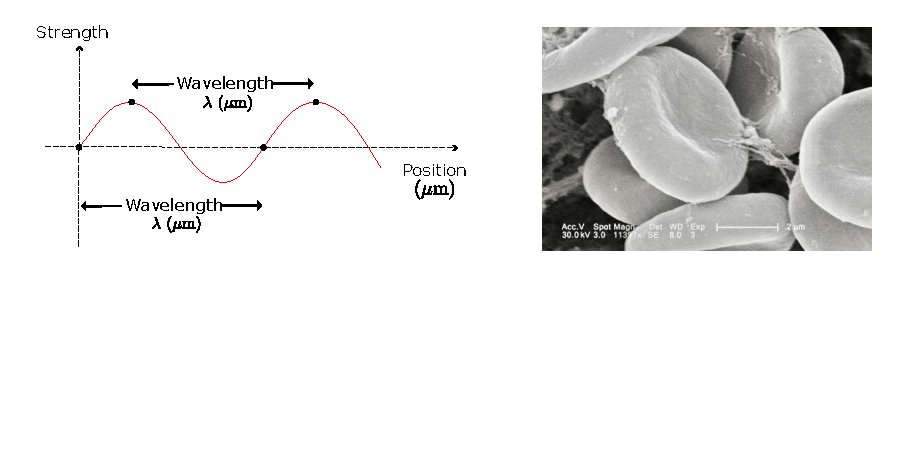
\includegraphics[width=0.9\textwidth]{images/04_scale-wavelength-rbc.pdf}
\end{center}
%
Now consider the rest of the electromagnetic spectrum.  We give the names to ranges of wavelength values: gamma-rays, X-rays, ultraviolet, visible, near-infrared, infrared/far-infrared, microwave, radio.   
	%
	\begin{itemize}
	\item Look up the wavelength ranges of these types of light and \underline{make a table}, putting all wavelengths in micrometer ($\mu$m).
	\item On the wavelength axis below (in log scale) show the range of each type of light.  [Notice that $\unit{10^0}{\micro\meter} = \unit{1}{\micro\meter}$ (and $10^{1} =10$, $10^{-1} = 1/10$), and that the midpoint between $1$ and $10$ on a logarithmic scale is 3.]
	\end{itemize}
	%
	%
\begin{center}
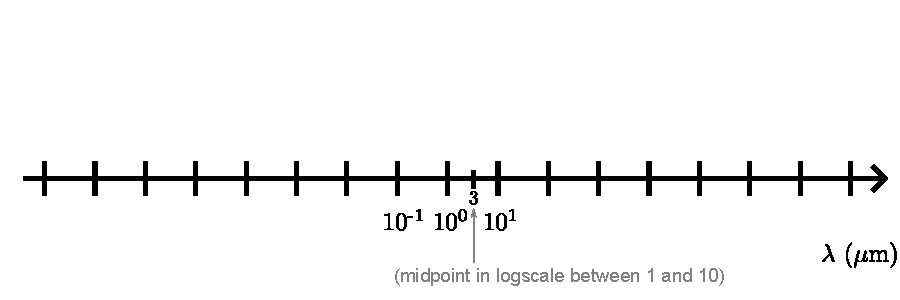
\includegraphics[width=0.9\textwidth]{images/04_EM-spectrum-logscale}
\end{center}

\subsection{Blackbody Radiation}

Any object that has internal energy will have a temperature greater than absolute zero ($\unit{0}{\kelvin} = -273\degree$C); and it turns out that any object with a temperature radiates light.    This phenomena is called {\bf blackbody radiation}.   There are a few key equations that describe the amount and wavelength of light emitted by blackbody radiators:
%
\begin{equation*}
\lambda_\text{peak} = \frac{\unit{2900}{\micro\meter \cdot \kelvin}}{T} \quad \quad \text{Wien's Law, wavelength of peak emission}
\end{equation*}
%
\begin{equation*}
F = \left( 6 \times 10^{-8} \, \frac{\text{J}/\text{s}}{\text{m}^2 \cdot \text{K}^4}\right) T^4 \quad \quad \text{Stefan-Boltzmann Law (total flux)}
\end{equation*}
%
\begin{equation*}
F_\lambda = \frac{F}{1.5 \times \lambda_\text{peak}} \quad \quad \text{Peak value of ``Spectral Flux''}
\end{equation*}
%
Our Sun is the most familiar example of a (nearly) ideal blackbody radiator.  It has a temperature of about \unit{6000}{\kelvin}.  What is the wavelength of the peak of its blackbody radiation?  What is its total flux?

\vspace{3cm}

A table is given below showing the spectral emission or sensitivities of equipment we will use in the lab today.  Fill in the last column with the temperatures corresponding to blackbody radiators with peaks at the wavelengths given (one temperature if a single value, two temperatures if a range is given). There is space for calculation examples below.
%
\begin{center}
\begin{tabular}{|l|l|l|}
\hline
Device & Wavelength range ($\mu$m) \hspace{1cm} & BB Temperatures \hspace{2cm} \\
\hline
\hline
% WRONG IN F2025???   
%Mileseey IR Camera & \unit{4.6}{\micro\meter} -- \unit{11.5}{\micro\meter} & \\
Mileseey IR Camera & \unit{8}{\micro\meter} -- \unit{14}{\micro\meter} & \\
\hline
ELP USB NIR (webcam) & \unit{0.4}{\micro\meter} -- \unit{1.0}{\micro\meter} & \\
\hline
ELP USB NIR (illuminators) & \unit{0.94}{\micro\meter} & \\
\hline
Andoer IR49S LED Panel & \unit{0.855}{\micro\meter} & \\
\hline
Andoer IR49S LED Panel & \unit{0.855}{\micro\meter} & \\
\hline
AKASO v50 elite action camera & \unit{0.40}{\micro\meter}  -- \unit{0.70}{\micro\meter} & \\
\hline
\end{tabular}
\end{center}
%

\vspace{4cm}


\section{Experiments and Activities}


\subsection{Observations of light}

We have equipment for observing light in the (far) infrared (the Mileseey camera); in the near infrared (NIR) (the ELP webcam); and the visual range (your eyes and the AKASO ``action camera'').  For the NIR (and comparisons between NIR and visual) you can put the cameras and objects under the cardboard box to get a dark environment.  Objects with a temperature (at your table, around the room) can serve as sources of infrared light.  The Andoer LED panel acts as a source of near IR light.

\vspace{0.25cm}

\noindent For each item of observation, \underline{make and document (with words and images) some observations}.  Some things to try, and questions to answer:
	%
	\begin{itemize}
	\item Use the infrared camera to observe objects and people (with their permission!) around the room.  
	\item Try to see the ``ghosts'' of warm objects when they are removed from another object (your hand on the table or wall).
	\item Spill a bit of water on the floor and see what it looks like.
	\item See if various lights change in the IR picture when on/off.
	\item What are warm objects and cold objects in the room \ldots anything surprising?  (Note the temperature output on the image itself).
	\item Place the security camera and the visual camera under the box with a ``stage'' (little block) and a ``performer'' (bath toy animal).  How do their view compare?
	\item Put the NIR LED panel in the box as well, and document the visual and NIR camera views.
	\item Can you see the NIR LEDs with your eye?  
	\item Can anything see the bulb in the TV remote when you press its buttons?
	\item How does the NIR webcam see things?  Is it the same idea as the IR camera?  How do such ``security cameras'' work, and why are they designed this way?
	\end{itemize}

\subsection{Observations of transmission of light}

Whether an object is called {\bf transparent} or {\bf opaque} turns out to be wavelength dependent.  What does this mean in plain language?

\vspace{5cm}

\noindent Now make some observations.  Some things to try and questions to answer:
	%
	\begin{itemize}
	\item Use the ``clear'' plastic window, with various sources and cameras.
	\item Use the silicon plates (be careful they are fragile, but you can put your fingers on them) with various sources and cameras.
	\item Try the glass in the doorway.
	\item Fill a small beaker with coke. Place an object (pencil?) in it and observe with your eyes, the action camera, and under the box with the NIR camera and/or the visible light camera, with and without the NIR LED panel.
	\item Try out the ``faraday cage'' and the AM/FM radio.  Two local stations are WGVU (88.5 MHz) and WOOD (1300 KHz).  What are the wavelengths of these broadcast stations (calculate using $c = \lambda f$, where the speed of light is $c = \unit{3 \times 10^8}{\meter/\second}$).
	\item Does the faraday cage affect cell-phone signals?
	\end{itemize}






 